\section{VeriFast}

Im Rahmen dieser Seminararbeit werden wir uns hauptsächlich mit dem Verifikationswerkzeug \emph{VeriFast} auseinandersetzen, dass in Form eines Prototypen an der KU Leuven ins Leben gerufen wurde und aktiv weiterentwickelt wird. VeriFast erlaubt die Verifikation von \emph{single-} und \emph{multithreaded} C und Java Programmen, welche mit zusätzlichen Annotationen für die Verifikation bestimmter Korrektheitseigenschaften ausgestattet sind. Die Annotationen stehen innerhalb von Kommentaren, wodurch der verifizierte C Code ohne zusätzliche Änderungen kompiliert werden kann. Während der Ausführung von VeriFast wird das Programm auf illegale Speicherzugriffe, beispielsweise durch Dereferenzierung von Null-Pointern oder durch Zugriff auf Speicherzellen außerhalb der Grenzen eines Arrays, sowie Fehler aufgrund nebenläufiger Ausführung geprüft. Darüber hinaus verifiziert VeriFast die annotierten Methoden-Kontrakte - d.h. es wird versucht zu zeigen, dass sich die Nachbedingung aus der Vorbedingung und der symbolischen Ausführung des Methodenrumpfs ergibt. Diesbezüglich wird im Back-End der SMT Solver \emph{Z3} von Microsoft verwendet. \cite{Jacobs2010}

\begin{figure}[!hbt]
	\centering
	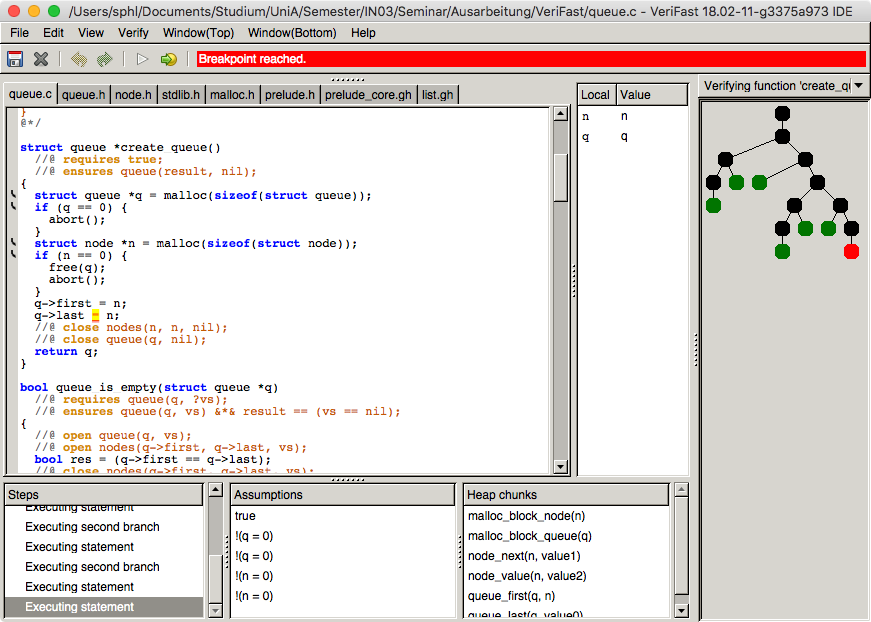
\includegraphics[width=0.8\linewidth]{verifast}
	\caption{VeriFast IDE}
	\label{fig:vfide}
\end{figure}

\noindent
Über die VeriFast IDE (siehe \vref{fig:vfide}) können Quellcodedateien editiert und Programme schrittweise/in einem Durchlauf verifiziert werden. Im Falle eines Fehlers werden diese innerhalb des Editors lokalisiert und anhand einer Statusmeldung dem Benutzer mitgeteilt. Wurde die Verifikation erfolgreich durchlaufen, so können abhängig von der ausgewählten Funktion die getesteten Pfade in Form eines Ausführungsbaums angezeigt werden. Zudem ermöglicht VeriFast über das Anklicken eines Blattknotens die Analyse einzelner Pfade. Die \emph{steps}-Auswahl listet hierbei die ausgeführten Schritte eines Pfades auf und erlaubt Sprünge zu vorherigen bzw. nachfolgenden Zuständen. Nebenan befinden sich die logischen Annahmen (\emph{assumptions} bzw. \emph{path constraints}), die sich aus den Annotationen und dem ausgeführten C Code ergeben. Eine Besonderheit der IDE ist die Anzeige der \emph{heap chunks}, welche abhängig vom Ausführungsschritt den symbolischen Zustand des Heap-Speichers darstellen. Darüber befindet sich eine weitere Auswahl, welche einen Überblick über die Zuordnung der lokalen Variablen auf deren symbolischen Werte gibt.

\subsection{Sprachkonstrukte}

In diesem Abschnitt werden einige (Sprach-)Konzepte vorgestellt die VeriFast für die Programmverifikation bereitstellt. Dabei werden vorzugsweise die Konzepte behandelt, welche für das Verständnis des Beispiels in \cref{subsec:queue} relevant sind. Weiterführende Konzepte und Beispiele können in \cite{Jacobs2017} nachgelesen werden.

\subsubsection{Induktive Datentypen}
\label{subsec:adt}

Ein wichtiges Hilfsmittel um die Korrektheit von Programme nachzuweisen, besteht in der Spezifikation von abstrakten Datentypen (ADT). Diese ermöglichen es, Eigenschaften und Operationen eines Datentyps auf einem höheren Abstraktionsniveau, d.h. unabhängig der konkreten Implementierung auf einem Computer, zu betrachten. Daraus resultierend können ADTs in der Programmverifikation als Repräsentanten für die Inhalte konkrete Datenstrukturen, wie beispielsweise Array oder einfach/doppelt verkettete Listen, eingesetzt werden. \cite[S. 265]{Saake2014}

VeriFast unterstützt den Einsatz von induktiven Datentypen, deren Instanzen über die Konkatenation von Konstruktoren (Konstruktorterm) gebildet werden. Die Spezifikation einer abstrakten Liste sieht dabei wie folgt aus.

\begin{lstlisting}
inductive list<t> = nil | cons(t, list<t>);
\end{lstlisting}

\noindent
In diesem Beispiel wurde eine generische Liste mit den Konstruktoren \texttt{nil} für die leere Liste und \texttt{cons} für die zusammengesetzte Liste, mit Kopfelement \texttt{t} und Restliste \texttt{list<t>}, definiert. Analog zu den meisten Programmiersprachen spezifiziert \texttt{<t>} den generischen Datentyp, wodurch Listen über \texttt{int}, \texttt{char}, \texttt{bool} etc. konstruiert werden können. So entspricht der Konstruktorterm \texttt{cons('a', cons('b', cons('c', nil)))} einer Liste mit der Zeichenfolge \texttt{<'a', 'b', 'c'>}.

\subsubsection{Fixpunkt Funktionen}

Neben den induktiven ADTs unterstützt VeriFast die Spezifikation von Fix\-punkt-Funktionen, wodurch spezifische Operation auf induktive Datentypen ausgeführt werden können. Diese werden mit \texttt{fixpoint} eingeleitet und erhalten über die Parameterliste einen oder mehrere ADTs. Im Funktionsrumpf kann entweder direkt eine \texttt{return}-Anweisung, welche die berechnete Eigenschaft an den Aufrufer zurückgibt, oder eine \texttt{switch}-Anweisung stehen. Letztere führt eine Fallunterscheidung bezüglich aller Konstruktoren von genau einem induktiven Argument (Fixpunkt) aus. Zudem prüft VeriFast jede Funktion auf Terminierung - d.h. im Falle eines rekursiven Aufrufs muss der neue Fixpunkt ein Teilterm des alten Konstruktorterms sein. \cite{Jacobs2010}

Ausgehend von der induktiven Liste in \cref{subsec:adt}, definieren wir die beiden Funktionen \texttt{head} und \texttt{tail}, welche das Kopfelement bzw. die Restliste des Fixpunkts \texttt{xs} zurückliefern.

\begin{lstlisting}
fixpoint t head<t>(list<t> xs) {
  switch (xs) {
    case nil: return default_value<t>;
    case cons(x, xs0): return x;
  }
}

fixpoint list<t> tail<t>(list<t> xs) {
  switch (xs) {
    case nil: return nil;
    case cons(x, xs0): return xs0;
  }
}
\end{lstlisting}

\noindent
Für den Konstruktor \texttt{cons(t, list<t>)} bindet VeriFast die entsprechenden Werte an die Variablen \texttt{x} und \texttt{xs0}, welche im Anschluss beliebig weiterverwendet werden können. Ein Sonderfall in diesem Beispiel ist der Konstruktor \texttt{nil} in \texttt{head}. Hierbei wird ein Defaultwert zurückgegeben, der je nach Anforderung und Datentyp unterschiedliche Werte annehmen kann.

Eine weitere bekannte Funktion auf Container-Datentypen ist \texttt{length}, welche in diesem Beispiel die Länge einer Liste rekursiv berechnet. Wurde ein Term ungleich \texttt{nil} übergeben, so wird dieser sukzessive abgebaut und zugleich die Länge um den Wert 1 erhöht. Der letzte Aufruf endet immer im \texttt{nil}-Konstruktor, welcher folgerichtig den die Länge 0 zurückgibt und damit die Berechnung abschließt.\footnote{\texttt{head}, \texttt{tail}, \texttt{length} und weitere Fixpunkt-Operationen auf \texttt{list<t>} sind Bestandteil der VeriFast-Bibliothek.}

\begin{lstlisting}
fixpoint int length<t>(list<t> xs) {
  switch (xs) {
    case nil: return 0;
    case cons(x, xs0): return 1 + length(xs0);
  }
}
\end{lstlisting}

\subsubsection{malloc\_block Einheiten}

Charakteristisch für C ist die dynamische Speicherverwaltung mittels \texttt{malloc} und \texttt{free}. Dadurch kann eine festgelegte Anzahl an Bytes angefordert und falls erfolgreich vom Betriebssystem alloziert, über einen Zeigen auf den Heap-Speicher angesprochen werden. Da C über keine automatische Garbage Collection (GC) verfügt, steht der Programmierer in der Pflicht den Speicherbereich manuell mit Hilfe von \texttt{free} zu räumen, falls dieser nicht mehr benötigt wird.

Den Zustand des Heap-Speichers gilt es auch bei der Verifikation von Programmen zu berücksichtigen. Hierbei legt VeriFast sogenannte \emph{chunks} auf dem symbolischen Heap ab, wann immer eine Datenstruktur während der symbolischen Ausführung alloziert wird. Instanzen die über \texttt{malloc} erzeugt wurden, erhalten dabei zusätzlich einen \texttt{malloc\_block} chunk. Über diesen Mechanismus kann vor der Freigabe überprüft werden, ob die zu löschende Instanz über einen gültigen \texttt{malloc\_block} Eintrag verfügt. \cite{Jacobs2010,Jacobs2017}

Das nachfolgende Listing zeigt die beiden C-Strukturen \texttt{node} und \texttt{queue}. Erstere stellt einen Knoten in einer einfach verketteten Liste dar, welche neben einer Character Variablen einen Zeiger auf das nächste Listenelement enthält. \texttt{queue} verfügt über zwei Zeiger die jeweils auf das erste bzw. letzte Element einer Liste/Warteschlange zeigen.

\noindent
\begin{minipage}{.45\textwidth}
\begin{lstlisting}
struct node {
  struct node *next;
  char value;
};
\end{lstlisting}
\end{minipage}
\hfill
\begin{minipage}{.45\textwidth}
\begin{lstlisting}
struct queue {
  struct node *first;
  struct node *last;
};
\end{lstlisting}
\end{minipage}

%\noindent
%Die Funktion create\_queue\footnote{\texttt{requires}, \texttt{ensures} und \texttt{close} werden erst in den darauffolgenden Abschnitten erklärt und können in diesem Beispiel übersprungen werden.} legt eine leere Queue auf dem Heap an, indem sie eine Queue alloziert und anschließend first und last den gleichen Knoten zu. Abschließend wird die Adresse der neu erstellten Queue an den Aufrufer zurückgeben.

\begin{lstlisting}
struct queue *create_queue()
  //@ requires true;
  //@ ensures queue(result, nil);
{
  struct queue *q = malloc(sizeof(struct queue));
  if (q == 0) { abort(); }
  struct node *n = malloc(sizeof(struct node));
  if (n == 0) { abort(); }
  q->first = n;
  q->last = n;
  //@ close nodes(n, n, nil);
  //@ close queue(q, nil);
  return q;
}
\end{lstlisting}

%\noindent
%Nach Ausführung dieser Funktion liegen folgende chunks auf dem Heap:

{\setlength\extrarowheight{5pt} % Vergroeßert den Zeilenabstand
\begin{table}[hbt!]
	\centering
	\begin{tabular}{|l|l|}
		\hline
		\rowcolor[HTML]{EFEFEF}
		% ----------------------------------------------------------------------------------------------------
		\textbf{Chunk}                   & \textbf{Beschreibung}                                     \\ \hline
		% ----------------------------------------------------------------------------------------------------
		\texttt{malloc\_block\_node(n)}  & Dynamisch allozierte Instanz \texttt{n}                   \\ \hline
		\texttt{malloc\_block\_queue(q)} & Dynamisch allozierte Instanz \texttt{q}                   \\ \hline
		\texttt{n->next |-> value1}      & Feld \texttt{next} hat symbolischen Wert \texttt{value1}  \\ \hline
		\texttt{n->value |-> value2}     & Feld \texttt{value} hat symbolischen Wert \texttt{value2} \\ \hline
		\texttt{q->first |-> n}          & Feld \texttt{first} zeigt auf Instanz \texttt{n}          \\ \hline
		\texttt{q->last |-> n}           & Feld \texttt{last} zeigt auf Instanz \texttt{n}           \\ \hline
		% ----------------------------------------------------------------------------------------------------
	\end{tabular}
\end{table}
}

\subsubsection{Prädikate}

\subsubsection{Kontrakte}

\subsubsection{Schleifeninvarianten}

\subsubsection{Lemma Funktionen}

\subsection{Verifikation -- Queue}
\label{subsec:queue}

\subsection{Praxis Fallstudien}

\subsubsection{Embedded Linux Network Management Software}

\subsubsection{Linux USB BP Keyboard Driver}

\subsection{Fazit}
